\renewcommand{\thesection}{A}
\newsection{Anhang}{appendix}
\pagestyle{appendix}
\newcommand{\figuretag}[1]{%
  \addtocounter{figure}{-1}%
  \renewcommand{\thefigure}{#1}%
}

\noindent\textbf{A.1:}\label{app:1}
\begin{figure}[H]\figuretag{A.1}
\centering
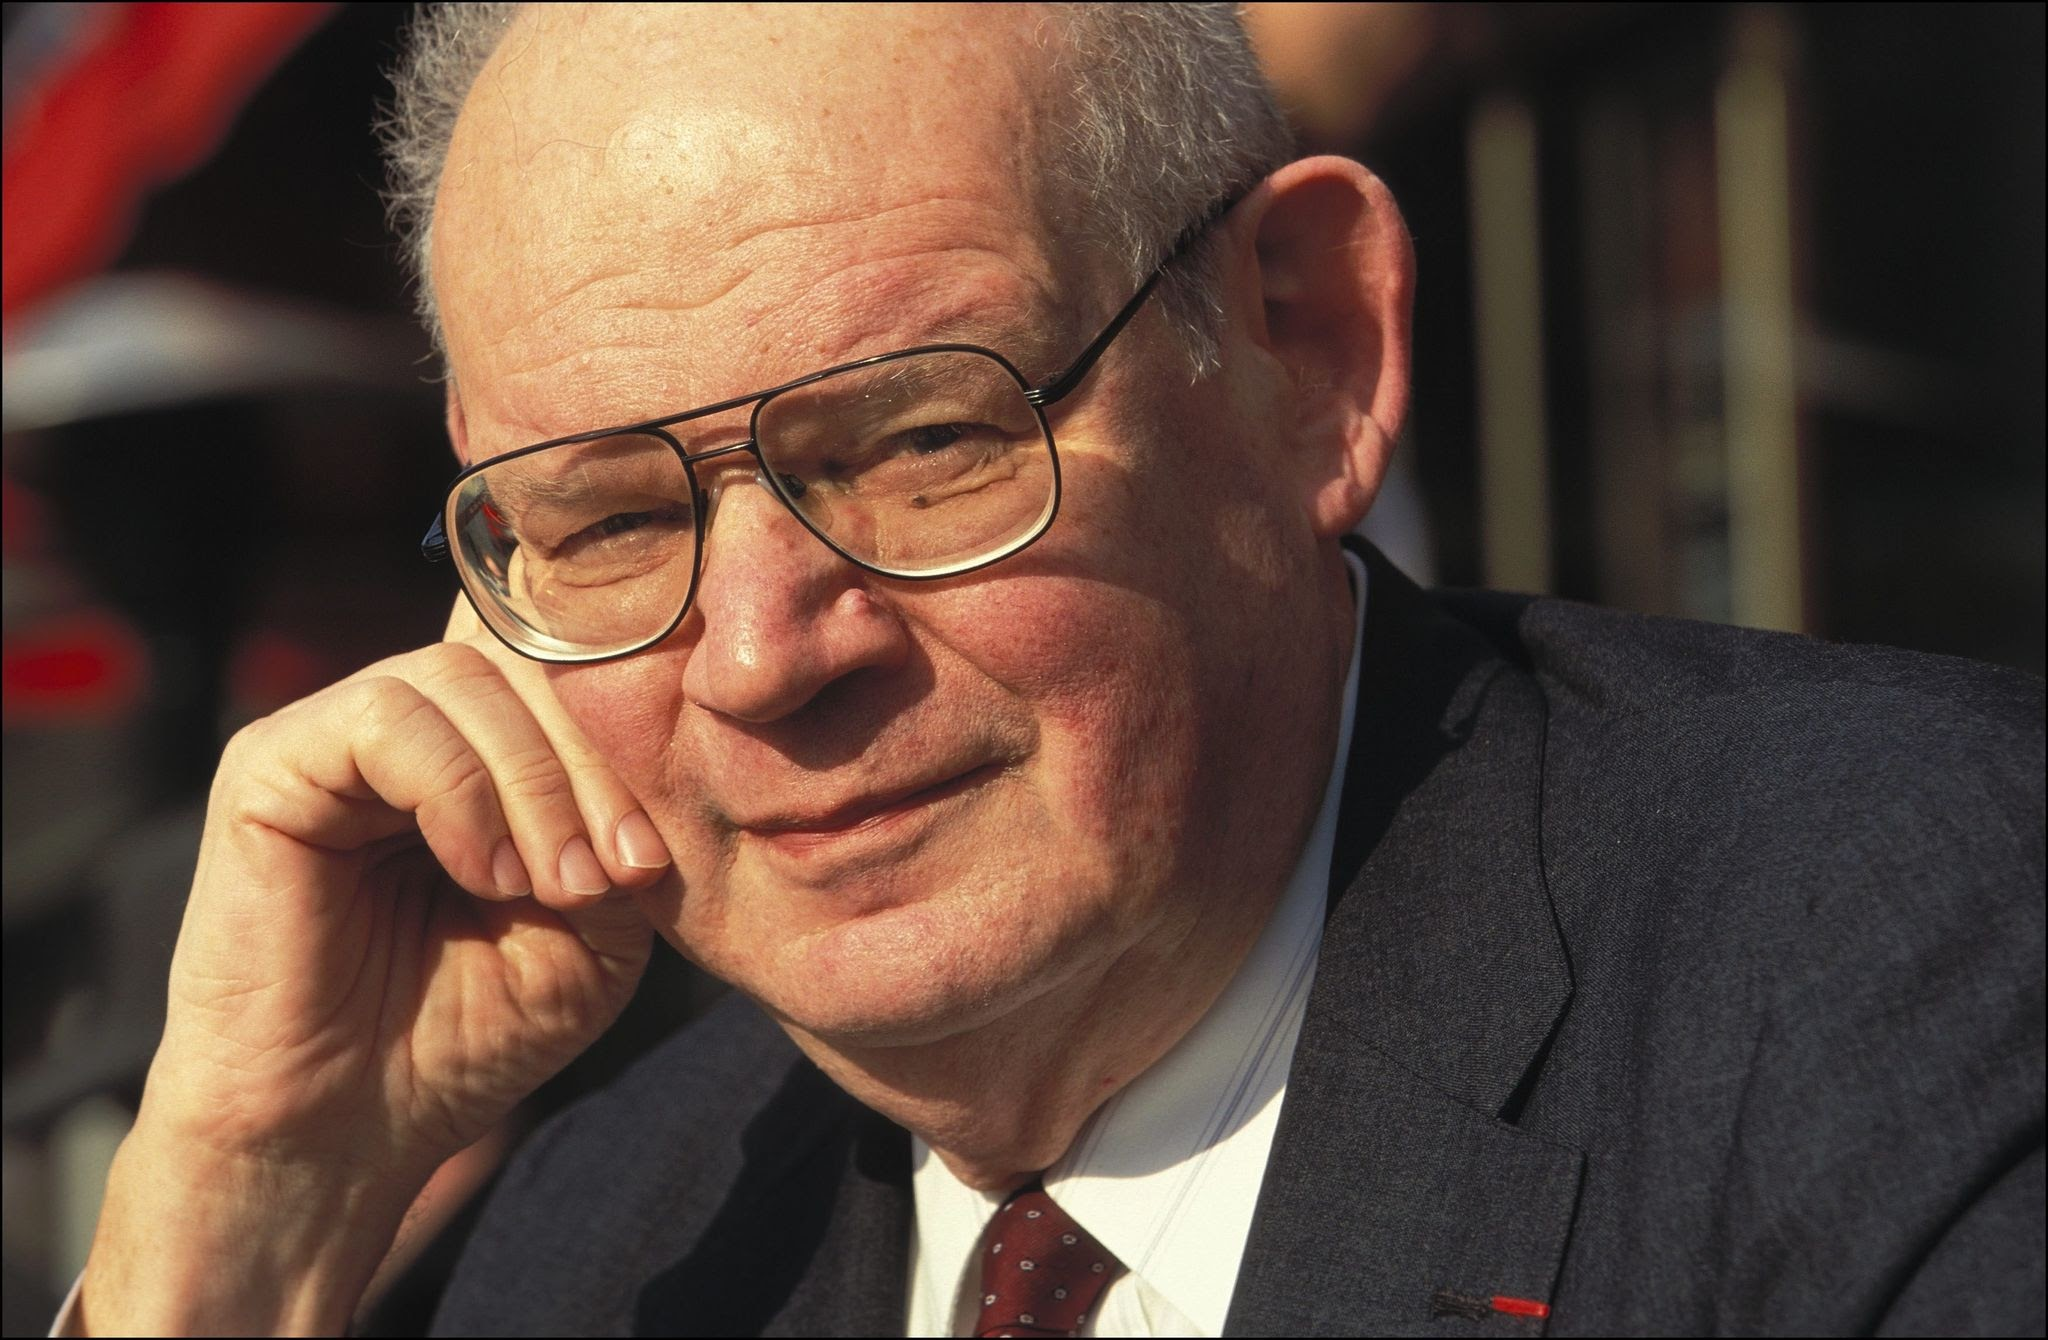
\includegraphics[width=0.7\textwidth]{images/benoit-mandelbrot}
\caption{Benoît Mandelbrot 1997 in Frankreich~\cite{gaillarde_benoit_1997}.}
\label{fig:benoit-mandelbrot-picture}
\end{figure}

\noindent\textbf{A.2:}\label{app:2}
\begin{equation}\tag{A.2}\label{eq:complex-numbers-multiplication}
  \begin{split}
    z_1 \cdot z_2 \\
    (a + bi) \cdot (c + di) \\
    =  c(a + bi) + di(a + bi) \\
    = ac + bci + adi + bdi^2 \\
    = ac + bci + adi - bd \\
    = ac - bd +(bc + ad)i
  \end{split}
\end{equation}

\noindent\textbf{A.3:}\label{app:3}
\begin{equation}\tag{A.3}\label{eq:complex-numbes-squaring}
  \begin{split}
    z_1^2
    = z_1 \cdot z_1 \\
    = (a + bi) \cdot (a + bi) \\
    = a \cdot (a + bi) + bi \cdot (a + bi) \\
    = a^2 + abi + abi - b^2 \\
    = a^2 - b^2 + 2abi
  \end{split}
\end{equation}

\noindent\textbf{A.4:}\label{app:4}
\begin{figure}[H]\figuretag{A.4}
  \centering
  \begin{tikzpicture}
    \begin{scope}[thick,font=\scriptsize]
      \fill[draw=black, fill=white] (0,0) circle (2);

      \draw [fill=black] (1,1.6) circle(0.05);
      \draw [fill=black] (-3,2.75) circle(0.05);
      \node at (1.75,1.85) {$ P_1(1|1.6i)$};
      \node at (-1.75,3) {$ P_2(-3|2.75i)$};

      \draw [->] (-4,0) -- (4,0) node [above left]  {$Re$};
      \draw [->] (0,-4) -- (0,4) node [below right] {$Im$};

      \foreach \n in {-3,...,-1,1,2,...,3}{
        \draw (\n, 3pt) -- (\n, -3pt)   node [below] {$\n$};
        \draw (3pt,\n) -- (-3pt,\n)   node [left] {$\n i$};
      }
    \end{scope}
  \end{tikzpicture}
  \caption{
    Einheitskreis mit dem Radius 2. Zu sehen ist der Punkt $P_1$, der im
    Einheitskreis liegt und Punkt $P_2$, der außerhalb des Einheitskreises liegt.
  }
  \label{fig:escape-radius}
\end{figure}

\noindent\textbf{A.5:}\label{app:5}
\begin{figure}[H]\figuretag{A.5}\label{fig:first-print-mandelbrot-set}
\centering
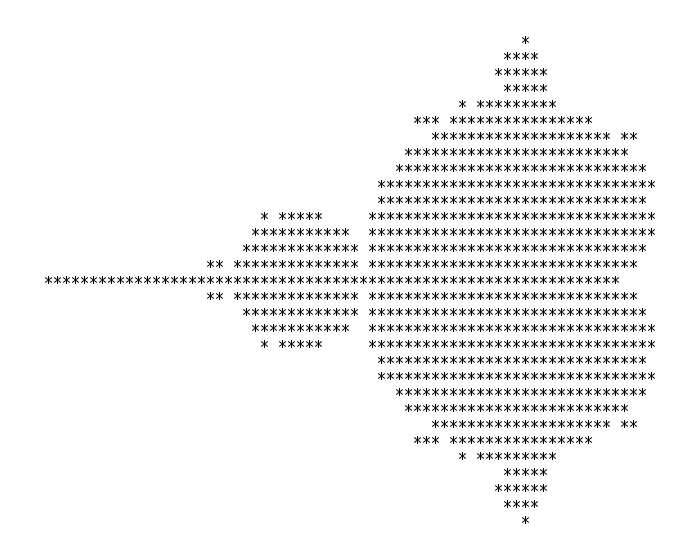
\includegraphics[width=0.7\textwidth]{images/Mandel}
\caption{
  Darstellung der ersten Drucks der Mandelbrot-Menge~\cite{elphaba_command-line_2007}.
}
\end{figure}
\newpage

\noindent\textbf{A.6:}\label{app:6}
\begin{figure}[H]\figuretag{A.6}\label{fig:mandelbrot-set-zoom-images}
  \centering
  \begin{minipage}[t]{0.40\textwidth}
    \centering
    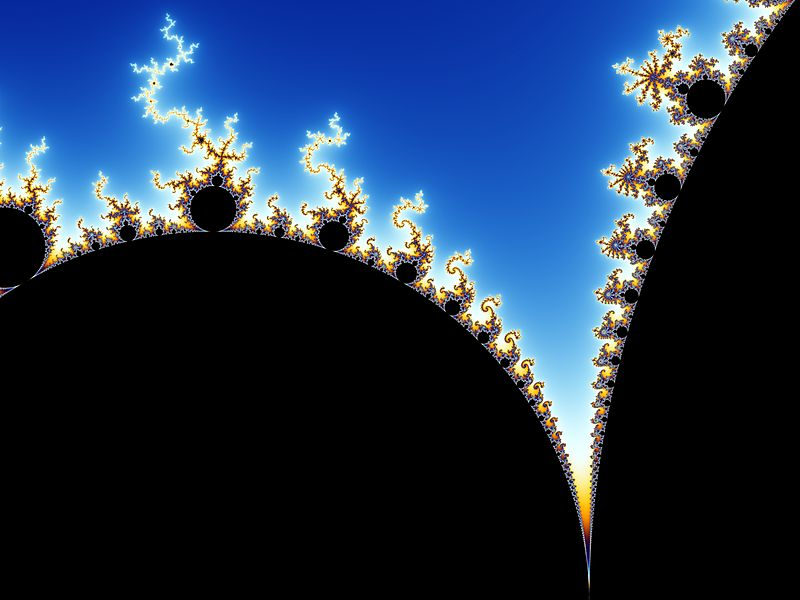
\includegraphics[width=\linewidth]{images/zoom/800px-Mandel_zoom_01_head_and_shoulder}
    \figuretag{A.6.1}
    \vspace*{-4ex}
    \caption{Spalte zwischen Kopf und K\"orper~\cite{beyer_partial_2005}}
    \label{app:6.1}
  \end{minipage}%
  \hspace{8ex}
  \begin{minipage}[t]{0.40\textwidth}
    \centering
    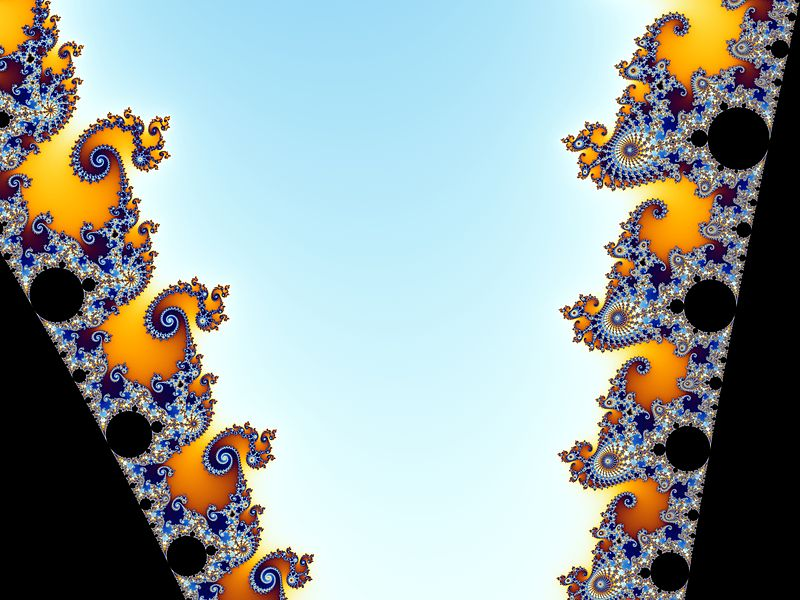
\includegraphics[width=\linewidth]{images/zoom/800px-Mandel_zoom_02_seehorse_valley}
    \figuretag{A.6.2}
    \vspace*{-4ex}
    \caption{\grqq Tal der Seepferdchen\glqq~\cite{beyer_partial_2005-1}}
    \label{app:6.2}
  \end{minipage}
  \\[4ex]
  \begin{minipage}[t]{0.40\textwidth}
    \centering
    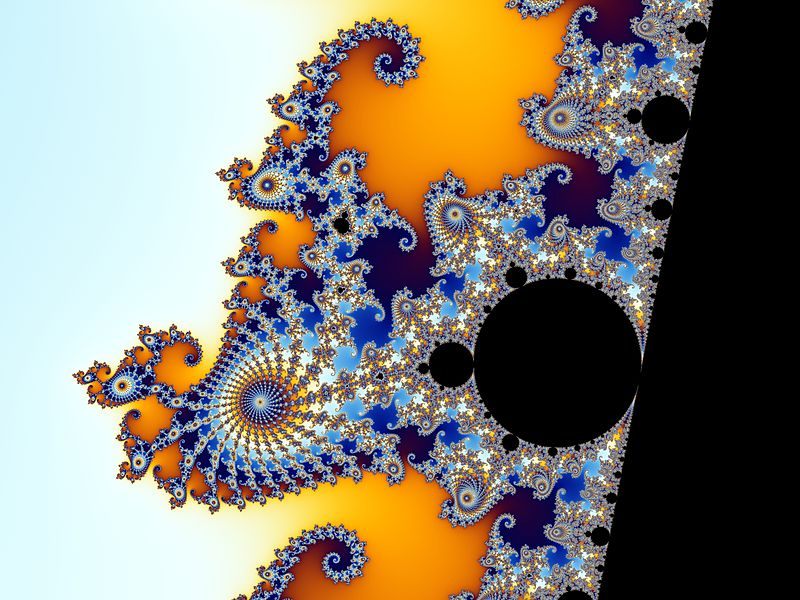
\includegraphics[width=\linewidth]{images/zoom/800px-Mandel_zoom_03_seehorse}
    \figuretag{A.6.3}
    \vspace*{-4ex}
    \caption{Rechts ein deformierter Satellit und links Misiurewicz-Punkt~\cite{beyer_partial_2005-2}}
    \label{app:6.3}
  \end{minipage}%
  \hspace{8ex}
  \begin{minipage}[t]{0.40\textwidth}
    \centering
    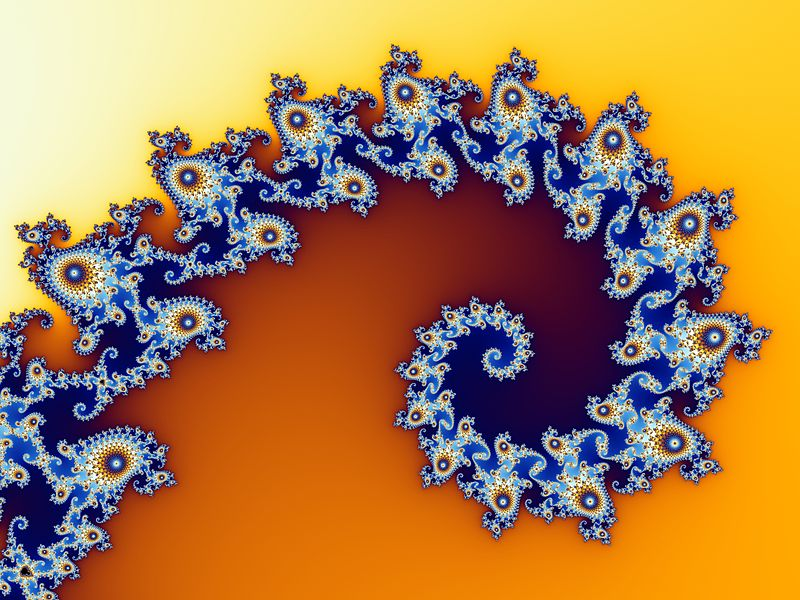
\includegraphics[width=\linewidth]{images/zoom/800px-Mandel_zoom_04_seehorse_tail}
    \figuretag{A.6.4}
    \vspace*{-4ex}
    \caption{Misiurewicz-Punkt~\cite{beyer_partial_2005-3}}
    \label{app:6.4}
  \end{minipage}
  \\[4ex]
  \begin{minipage}[t]{\textwidth}
    \centering
    
\includegraphics[width=0.45\linewidth]{images/zoom/800px-Mandel_zoom_08_satellite_antenna}
    \figuretag{A.6.5}
    \vspace*{-2ex}
    \caption{Satellit mit ähnlicher Struktur wie das Apfelm\"annchen~\cite{beyer_partial_2005-4}}
    \label{app:6.5}
  \end{minipage}
\end{figure}

\noindent\textbf{A.7:}\label{app:7}
\begin{figure}[H]\figuretag{A.7}
\centering
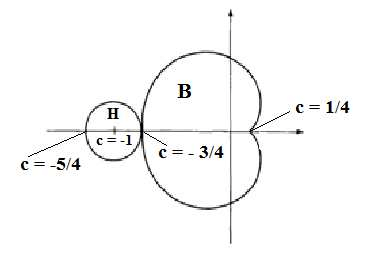
\includegraphics[width=0.5\textwidth]{images/bodyHeadMandelbrotSet}
\caption{
  K\"orper (B) und Kopf (H) der Mandelbrot-Menge~\cite{mahanta_mandelbrot_2016}.
}
\label{fig:body-and-head-of-mandelbrot-set}
\end{figure}

\noindent\textbf{A.8:}\label{app:8}
\vspace*{-2ex}
\begin{figure}[H]\figuretag{A.8}
\centering
\begin{minipage}[t]{0.48\textwidth}
  \centering
  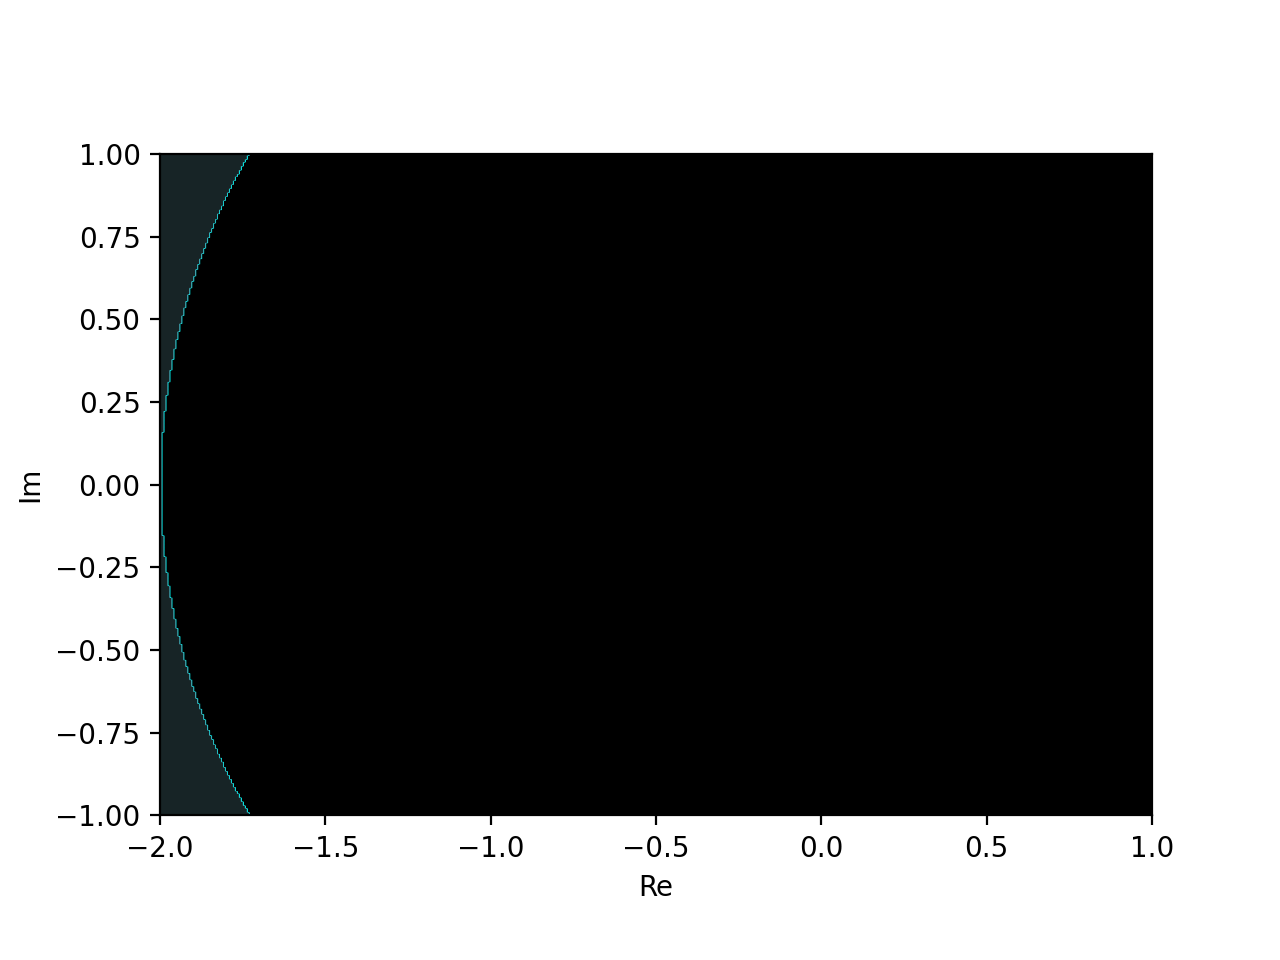
\includegraphics[width=\linewidth]{images/maxBorder/1}
  \figuretag{A.8.1}
  \vspace*{-8ex}
  \caption{Generiertes Bild mit einer Iterationsgrenze von $1$}
  \label{app:8.1}
\end{minipage}%
\hspace{2ex}
\begin{minipage}[t]{0.48\textwidth}
  \centering
  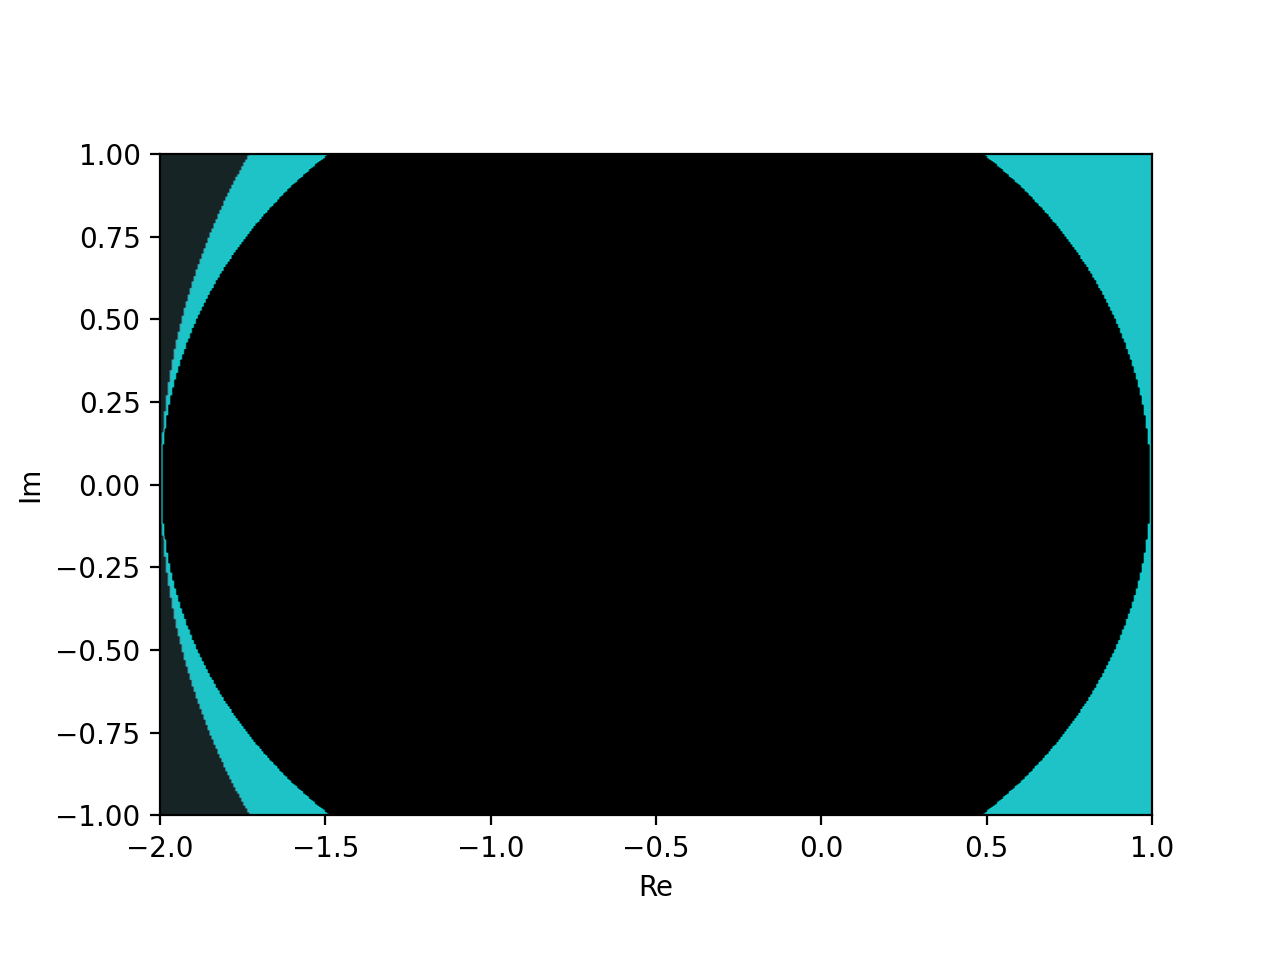
\includegraphics[width=\linewidth]{images/maxBorder/2}
  \figuretag{A.8.2}
  \vspace*{-8ex}
  \caption{Generiertes Bild mit einer Iterationsgrenze von $2$}
  \label{app:8.2}
\end{minipage}
\begin{minipage}[t]{0.48\textwidth}
  \centering
  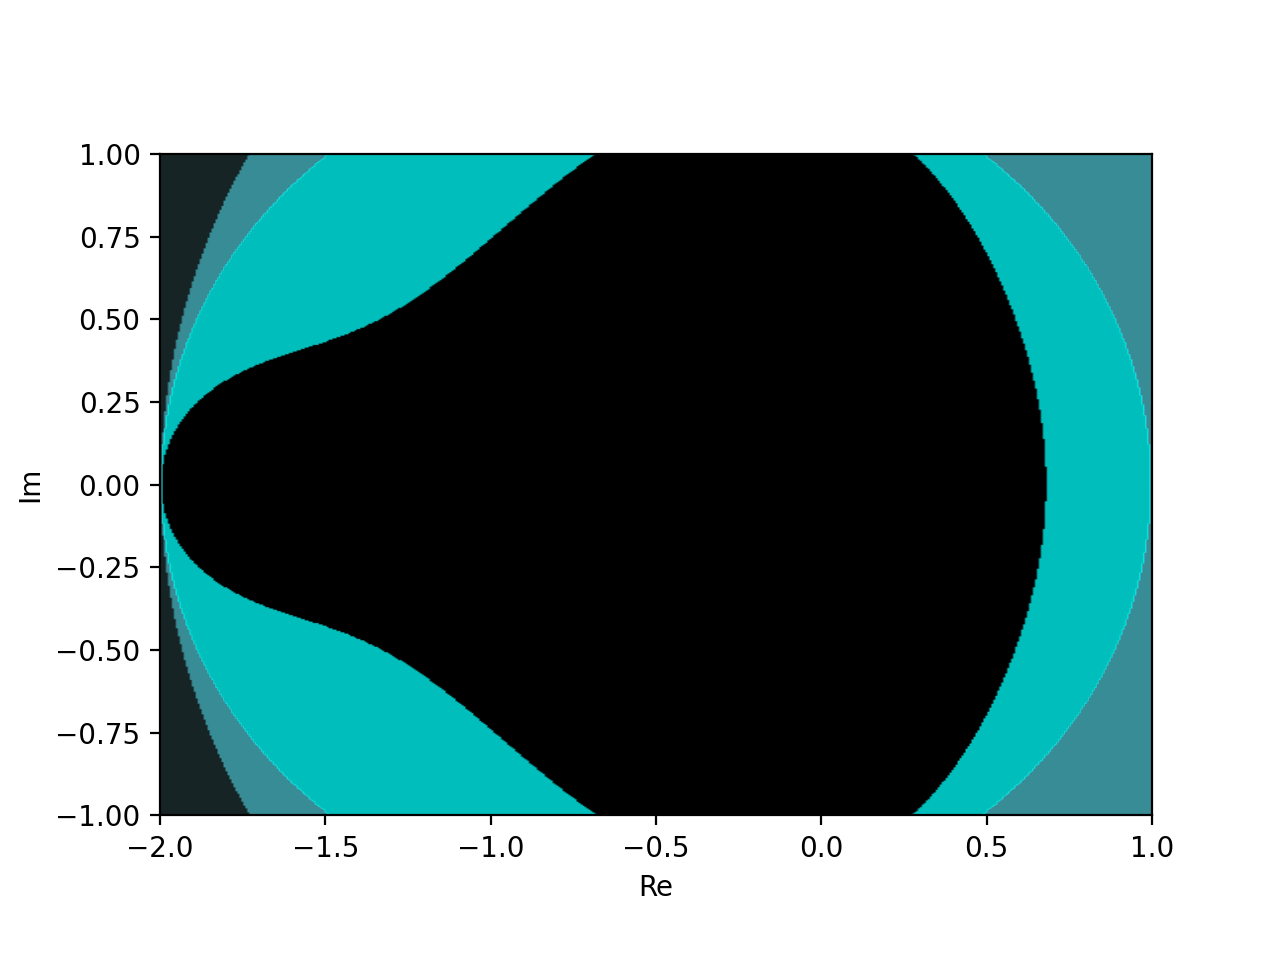
\includegraphics[width=\linewidth]{images/maxBorder/3}
  \figuretag{A.8.3}
  \vspace*{-8ex}
  \caption{Generiertes Bild mit einer Iterationsgrenze von $3$}
  \label{app:8.3}
\end{minipage}%
\hspace{2ex}
\begin{minipage}[t]{0.48\textwidth}
  \centering
  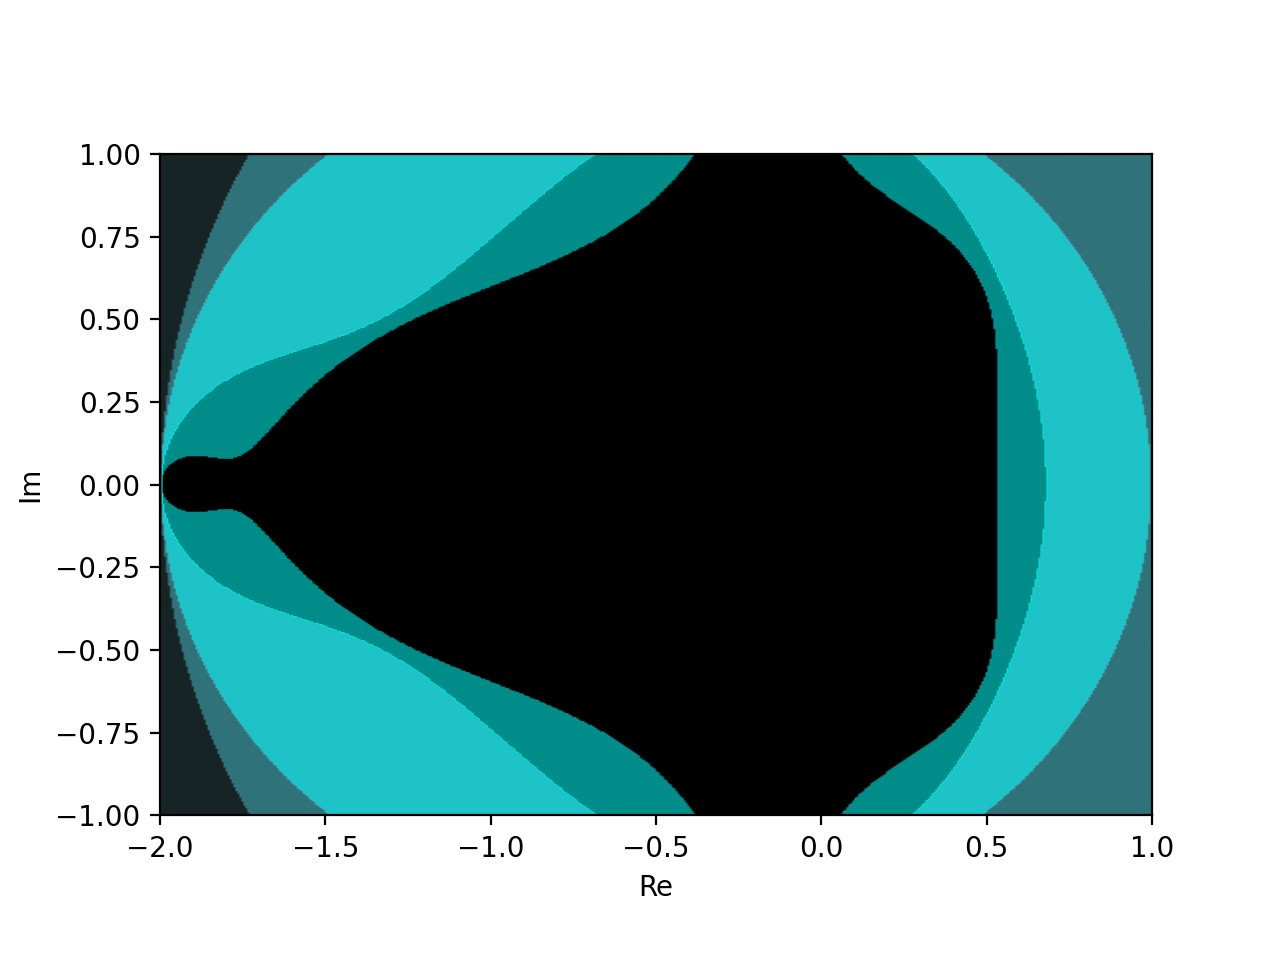
\includegraphics[width=\linewidth]{images/maxBorder/4}
  \figuretag{A.8.4}
  \vspace*{-8ex}
  \caption{Generiertes Bild mit einer Iterationsgrenze von $4$}
  \label{app:8.4}
\end{minipage}
\label{fig:mandelbrot-set-max-border-1}
\end{figure}
\newpage

\begin{figure}[H]\figuretag{A.8}
\centering
\begin{minipage}[t]{0.48\textwidth}
  \centering
  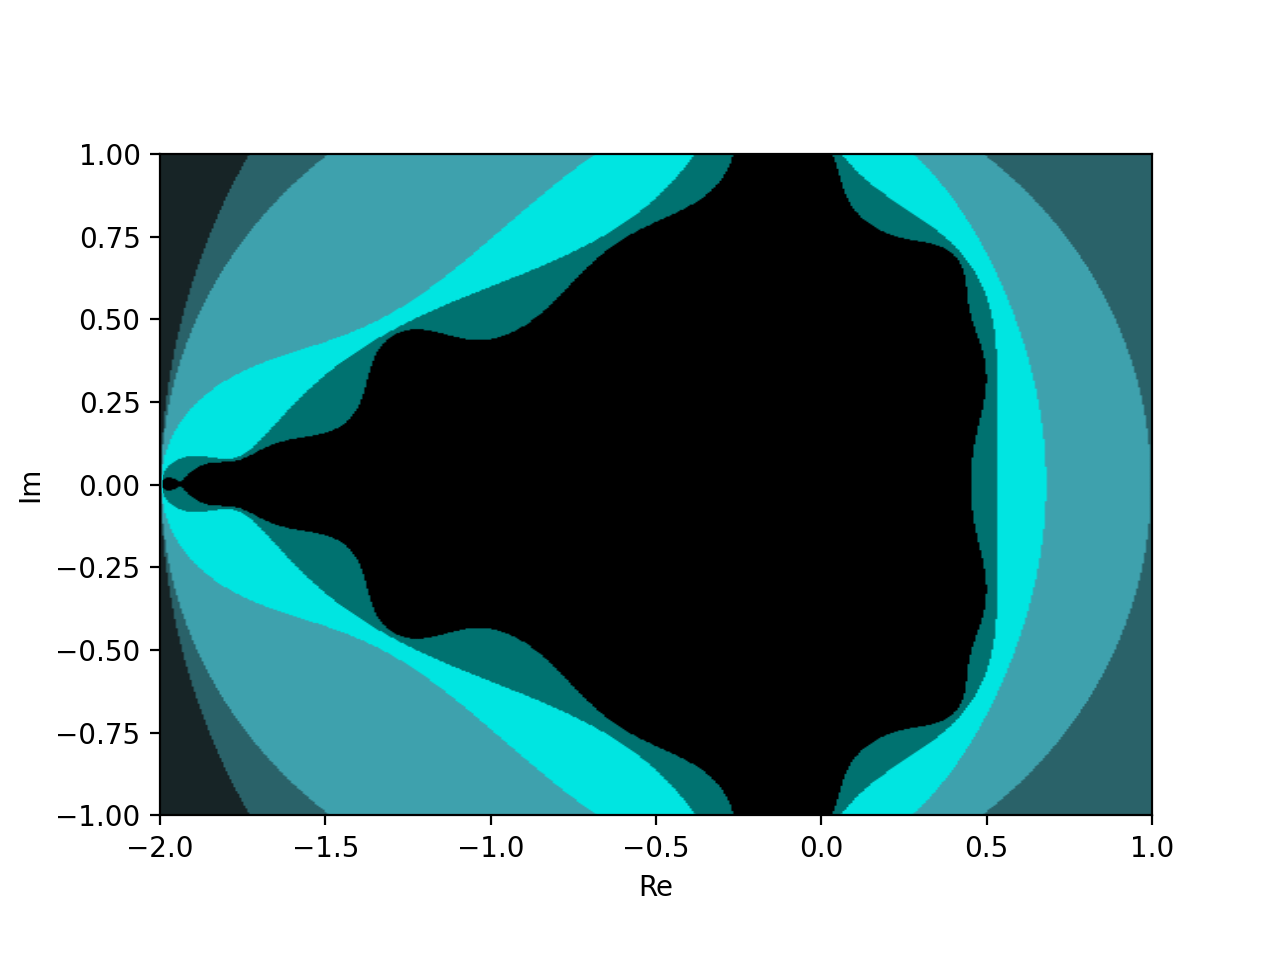
\includegraphics[width=\linewidth]{images/maxBorder/5}
  \figuretag{A.8.5}
  \vspace*{-8ex}
  \caption{Generiertes Bild mit einer Iterationsgrenze von $5$}
  \label{app:8.5}
\end{minipage}%
\hspace{2ex}
\begin{minipage}[t]{0.48\textwidth}
  \centering
  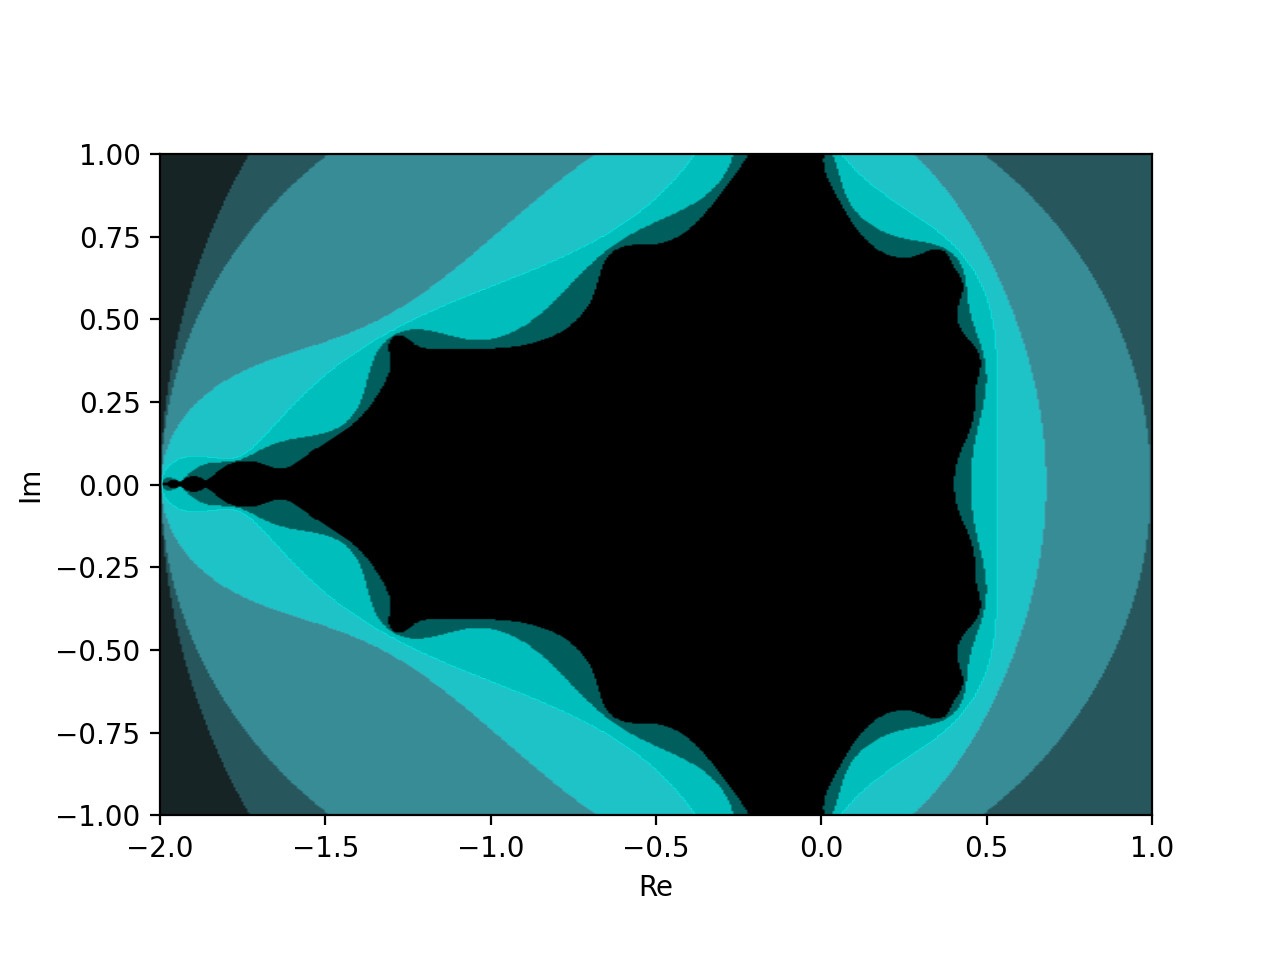
\includegraphics[width=\linewidth]{images/maxBorder/6}
  \figuretag{A.8.6}
  \vspace*{-8ex}
  \caption{Generiertes Bild mit einer Iterationsgrenze von $6$}
  \label{app:8.6}
\end{minipage}
\begin{minipage}[t]{\textwidth}
  \centering
  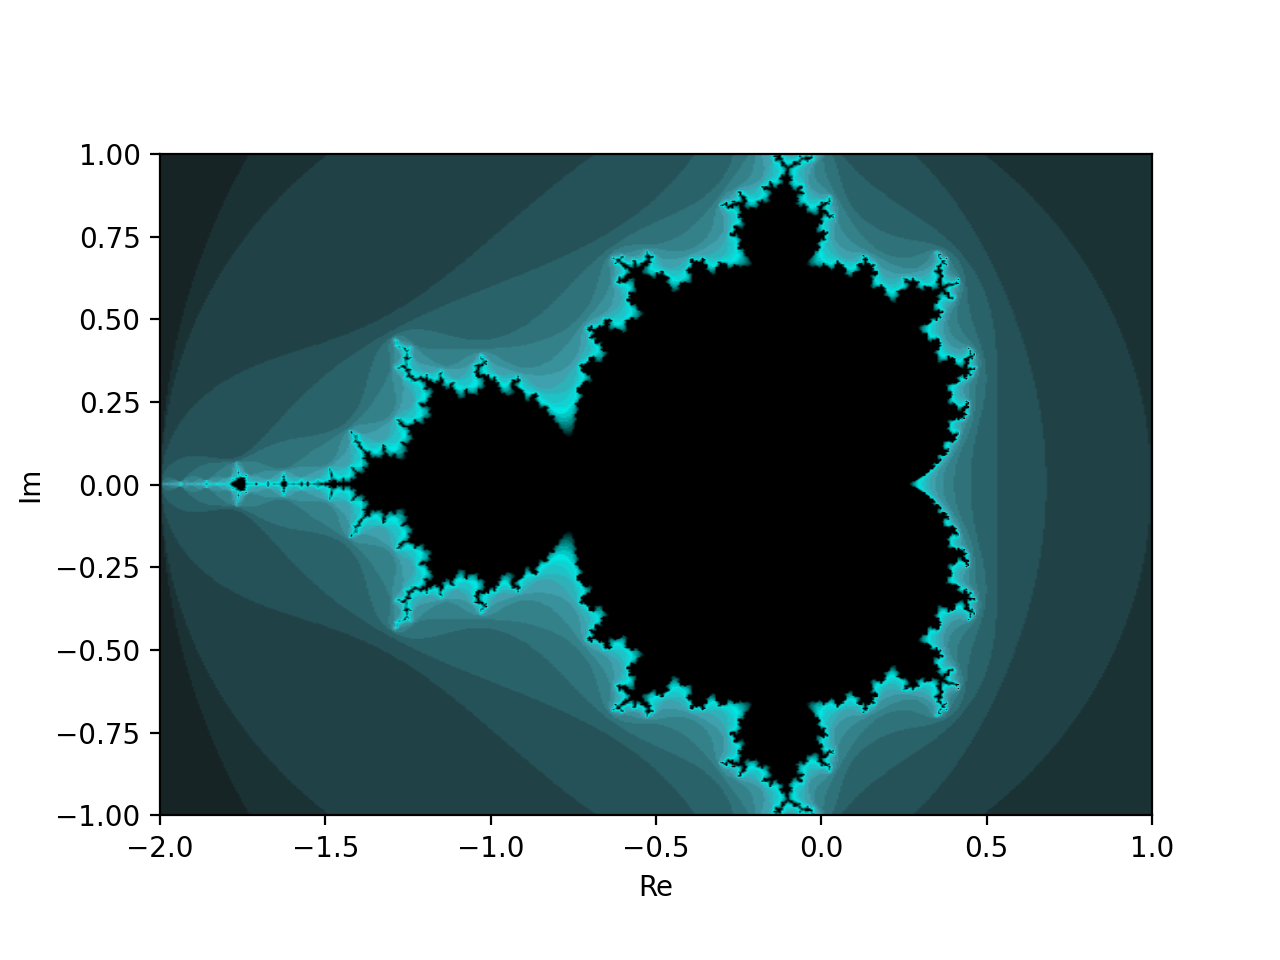
\includegraphics[width=0.48\linewidth]{images/maxBorder/20}
  \figuretag{A.8.7}
  \vspace*{-4ex}
  \caption{Generiertes Bild mit einer Iterationsgrenze von $20$}
  \label{app:8.7}
\end{minipage}
\label{fig:mandelbrot-set-max-border-2}
\end{figure}

\noindent\textbf{A.9:}\label{app:9}
\begin{figure}[H]\figuretag{A.9}
\centering
\begin{minipage}[t]{0.30\textwidth}
  \centering
  
\includegraphics[width=0.5cm, height=3cm]{images/simple_color_map}
  \figuretag{A.9.1}
  \caption{Simple HSV-Colormap mit einem linearen Farbverlauf}
  \label{app:9.1}
\end{minipage}%
\hfill
\begin{minipage}[t]{0.30\textwidth}
 \centering
 
\includegraphics[width=0.5cm, height=3cm]{images/used_color_map}
 \figuretag{A.9.2}
 \caption{Komplexe HSV-Colormap mit vier verschiedenen Ankerpunkten}
 \label{app:9.2}
\end{minipage}%
\hfill
\begin{minipage}[t]{0.30\textwidth}
 \centering
 
\includegraphics[width=0.5cm, height=3cm]{images/complex_color_map}
 \figuretag{A.9.3}
 \caption{Komplexe HSV-Colormap mit vielen unterschiedlichen Ankerpunkten}
 \label{app:9.3}
\end{minipage}
\label{fig:color-maps}
\end{figure}

\noindent\textbf{A.10:}\label{app:10}
\vspace*{1em}
\lstinputlisting[
  language=Python,
  label={lst:generation-code},
  backgroundcolor=\color{white},
  basicstyle=\linespread{0.6}\footnotesize,
  breaklines=true,
  captionpos=b,
  commentstyle=\color{mygreen},
  keywordstyle=\color{blue},
  stringstyle=\color{mymauve},
  caption={[Caption for LOF]
    Python-Code zur Generierung der\hyperref[fig:mandelbrot-set]{
      Abbildung \ref{fig:mandelbrot-set}
    }
  }
]{sections/mathematicalConsideration/generate.py}

\vfill
\centering
\noindent\textbf{Weitere Anhänge und benutzte Webseiten:}